\documentclass[a4paper,titlepage]{report}
\usepackage{fullpage}
\usepackage{titlesec}
\usepackage{array}
\usepackage{url}
\usepackage{float}
\usepackage{listings}
\usepackage{enumitem}
\usepackage{graphicx}
\usepackage{verbatim}
\usepackage[dutch]{babel}
\usepackage{hyperref}
\usepackage[toc,nonumberlist,style=altlist,translate=true]{glossaries}
\usepackage{glossaries-babel}
\makeglossaries

% Nummering voor subsubs en pars
\renewcommand{\thesubsubsection}{\arabic{subsubsection}}
\renewcommand{\theparagraph}{\thesubsubsection.\arabic{paragraph}}

\lstset{
    numbers=none,
    frame=shadowbox,
    identifierstyle=\ttfamily,
    keywordstyle=\color[rgb]{0,0,0},
    commentstyle=\color[rgb]{0,0,0},
    stringstyle=\color[rgb]{0,0,0},
    xleftmargin=30pt,
    xrightmargin=10pt,
    showstringspaces=false,
    breaklines=true,
    escapeinside={(*@}{@*)}
}

\makeatletter
% Label with name
\def\namedlabel#1#2{
  \label{#1}
  \begingroup
   \def\@currentlabel{#2}%
   \label{#1:name}\endgroup
}

% Label with name and displayed
\def\nameddisplayedlabel#1#2{
  \label{#1}
  \begingroup
   \def\@currentlabel{#2}%
   \label{#1:name}\endgroup
   \textbf{#2}\hfill\\
}

% Reference with name
\def\namedref#1{\ref{#1} \ref{#1:name}}
\makeatother



\title{Deliverance:\\ Requirements\\ Milestone 1\\ Iteratie 3\\ RC 3}
\author{Lucas de Vries \& Stefan van Wouw}
\begin{document}
\maketitle


% Glossary entries
\newglossaryentry{def:stuk}{name=Stuk,text=stuk,plural=stukken, description={Een
archiefstuk, boek, brochure, tijdschrift, of andere ge\"indexeerde eenheid uit
het archief of bibliotheek van het IISG. Indien een archief niet ge\"indexeerd
is, wordt het hele archief als \'e\'en stuk beschouwd. Alle stukken zijn
analoog, d.w.z. fysiek aanwezig, tenzij er wordt gesproken over digitale
stukken. Zowel de algemene metadata over een stuk, als een specifiek exemplaar
kan een `stuk' worden genoemd. Voorbeeld van onderscheid: Er zijn een aantal
exemplaren van een boek aanwezig. De contactinformatie, titel, inzage
restricties e.d. staan opgeslagen in de algemene metadata van het stuk. De
locatie informatie, gebruiksrestrictie (open/dicht) en status (uitgeleend of
niet) zijn per exemplaar opgeslagen}}
\newglossaryentry{def:hrb}{name=Hoog Resolutie Bestand,text=hoog resolutie
bestand,plural=hoge resolutie bestanden,description={Een afbeelding met hoge
resolutie/kwaliteit. Exacte resolutie/kwaliteit is door een extern systeem
bepaald (De Shared Object Repository)}}
\newglossaryentry{def:pdf}{name=PDF,description={Portable Document Format; een
veelgebruikt bestandsformaat om documenten in op te slaan}}
\newglossaryentry{def:ftp}{name=FTP,description={File Transfer Protocol; een
gestandaardiseerd protocol om bestanden uit te wisselen tussen verschillende
computers}}
\newglossaryentry{def:use-case}{name=Use Case,text=use case,description={Een
bepaalde sequentie van handelingen die de interactie tussen een gebruiker en een
systeem weergeeft}}
\newglossaryentry{def:ui}{name=User Interface,text=user
interface,description={Deel van het systeem dat de interactie tussen de
gebruiker en het systeem mogelijk maakt}}
\newglossaryentry{def:fr}{name=Functionele Requirement,text=functionele
requirement,description={Eis die beschrijft wat het systeem moet kunnen. Dit
type eis is direct af te leiden uit de probleemstelling}}
\newglossaryentry{def:nfr}{name=Niet-Functionele Requirement,text=niet-functionele
requirement,description={Eis die de randvoorwaarden aan het
systeem die niet direct uit de probleemstelling zijn af te leiden beschrijft}}
\newglossaryentry{def:bezoeker}{name=Bezoeker,text=bezoeker,description={Een persoon
die te gast is bij het IISG om danwel stukken in te zien, danwel reproducties te
bestellen. De bezoeker kan zowel via het internet, als op locatie een service
van het IISG gebruiken}}
\newglossaryentry{def:medewerker}{name=Medewerker,text=medewerker,description={Een
magazijn-,
studiezaal-, of reproductiemedewerker}}
\newglossaryentry{def:studiezaalmedewerker}{name=Studiezaalmedewerker,text=studiezaalmedewerker,
description={Een medewerker van de studiezaal die bezoekers te woord staat en
stukken uitleent ter inzage}}
\newglossaryentry{def:magazijnmedewerker}{name=Magazijnmedewerker,text=magazijnmedewerker,
description={Een medewerker die stukken van en naar het magazijn brengt}}
\newglossaryentry{def:reproductiemedewerker}{name=Reproductiemedewerker,text=reproductiemedewerker,
description={Een medewerker die zorgt dat de aanvragen voor reproductie worden
afgehandeld}}
\newglossaryentry{def:uitleenstatus}{name=Uitleenstatus,text=uitleenstatus,description={Een
status van een stuk dat aangeeft waar een bepaald exemplaar van een stuk zich op dit moment bevindt.
Mogelijke waarden zijn: Beschikbaar, Aangevraagd, Uitgeleend, Teruggebracht}}
\newglossaryentry{def:wachtnummer}{name=Wachtnummertje,text=wachtnummertje,description={Een
nummer dat kan worden gebruikt om een bezoeker in een wachtrij te plaatsen. Als
de bezoeker een aanvraag ter inzage doet krijgt hij/zij dit nummer. Als de
stukken uit het magazijn zijn gehaald wordt het wachtnummer meegedeeld en kan de
bezoeker de stukken komen ophalen}}
\newglossaryentry{def:iDeal}{name=iDeal,description={Veelgebruikte Nederlandse
online betalingsmethode}}
\newglossaryentry{def:contactpersoon}{name=Contactpersoon,text=contactpersoon,description={Persoon
waarmee contact dient te worden opgenomen indien er een inzage restrictie op een
archief(stuk) rust}}
\newglossaryentry{def:metadata}{name=Metadata,text=metadata,description={Gegevens
over andere data. Denk aan de uitleenstatus, of inzage restrictie die een stuk
kan hebben}}
\newglossaryentry{def:inzage-restrictie}{name=Inzage Restrictie,text=inzage
restrictie,description={Restrictie wat betreft de inzage. Stukken kunnen `Open'
zijn, dan mag iedereen ze inzien, en dan mogen er ook reproducties van worden
gemaakt. `Restricted' geeft aan dat een stuk beperkt mag worden ingezien, de
exacte beperkingen zijn in de algemene metadata van een stuk vastgelegd (niet
per exemplaar). `Closed' geeft aan dat de stukken helemaal niet in mogen worden
gezien}}
\newglossaryentry{def:gebruiksrestrictie}{name=Gebruiksrestrictie,text=gebruiksrestrictie,
description={Beperking wat betreft het gebruik van een stuk. Het kan
bijvoorbeeld zijn dat alleen de microfilm mag worden uitgeleend en het origineel
niet. Dit is aangegeven per exemplaar}}
\newglossaryentry{def:embargodatum}{name=Embargodatum,text=embargodatum,description={Datum
waarna een stuk vrij wordt gegeven voor inzage. De inzage restrictie zal dan
automatisch naar `Open' veranderen}}
\newglossaryentry{def:framework}{name=Framework,text=framework,description={Een
raamwerk aan software componenten dat standaard-oplossingen biedt voor bepaalde
handelingen die vaak worden uitgevoerd bij het schrijven van software.
Voorbeeld: Django is een framework dat standaard-oplossingen biedt voor het
schrijven van een web-applicatie in de programmeertaal Python}}
\newglossaryentry{def:library}{name=Library,text=library,plural=libraries,
description={Een bibliotheek aan software componenten, welke gebruikt kan worden
bij het schrijven van andere software}}
\newglossaryentry{def:open-source}{name=Open Source,text=open
source,description={Een term gebruikt om aan te duiden dat de broncode van de
software voor iedereen toegankelijk is}}
\newglossaryentry{def:web-interface}{name=Web Interface,text=web
interface,description={User interface toegankelijk via een webbrowser, \emph{zie
User Interface}}}
\newglossaryentry{def:aanvraag}{name=Aanvraag,text=aanvraag,plural=aanvragen,description={Een
bezoeker kan een aanvraag doen om bepaalde stukken in te zien. Een aanvraag is
dus een verzameling stukken die gereserveerd danwel uitgeleend zijn voor inzage
door een bezoeker}}
\newglossaryentry{def:rechthebbende}{name=Rechthebbende,text=rechthebbende,description={De
persoon die eigenaar is van een verzameling van stukken/archief. Dit is in vele
gevallen ook de contactpersoon}}
\newglossaryentry{def:actor}{name=Actor,text=actor,description={Een type
gebruiker van het systeem (bijv. bezoeker of studiezaalmedewerker)}}
\newglossaryentry{def:reservering}{name=Reservering,text=reservering,plural=reserveringen,
description={\emph{Zie Aanvraag}}}
\newglossaryentry{def:preconditie}{name=Preconditie,text=preconditie,
description={Gegeven conditie die geldt voor aanvang van een reeks acties
(zoals een use case)}}
\newglossaryentry{def:postconditie}{name=Postconditie,text=postconditie,
description={Gegeven conditie die geldt na het uitvoeren van een reeks
acties (zoals een use case)}}
\newglossaryentry{def:api}{name=API,description={Application Programming
Interface; Een verzameling functies om de services die een bibliotheek of ander
programma biedt te kunnen gebruiken/aanroepen}}
\newglossaryentry{def:mvc}{name=MVC,description={Model-View-Controller;
Ontwerppatroon waarbij een duidelijke scheiding is gemaakt tussen de stukken
code die de data beheert (Model), de stukken code die zorgen voor de
presentatie(View), en de code die de logica van het programma bevat (Controller)}}
\newglossaryentry{def:vufind}{name=VuFind,description={Zoeksysteem veelal
gebruikt om catalogi te doorzoeken}}
\newglossaryentry{def:oai}{name=OAI-PMH,text=OAI,description={Open Archives
Initiative Protocol for Metadata Harvesting; Protocol om metadata tussen grote
archiefinstellingen uit te wisselen. Dit protocol is ge\"implementeerd door het
IISG (api.iisg.nl)}}
\newglossaryentry{def:sor}{name=SOR,description={Shared Object Repository; Een
extern systeem waar gedigitaliseerde stukken in worden opgeslagen}}
\newglossaryentry{def:rest}{name=REST,description={Representational State
Transfer; Een architecturele stijl om websites op te bouwen. Per URL kunnen
maximaal 4 verschillende request methoden worden gebruikt: GET om data van een
bepaalde URL locatie op te vragen, POST om data onder de gespecificeerde URL aan
te maken, PUT om data op de exact opgegeven locatie aan te maken/overschrijven,
en DELETE om de data op de locatie te verwijderen}}
\newglossaryentry{def:json}{name=JSON, description={JavaScript Object Notation;
Manier van noteren van Javascript objecten}}
\newglossaryentry{def:pid}{name=PID,description={Persistant Identifier; Een
persistente unieke code die gebruikt kan worden om bepaalde objecten (in dit
geval: stukken) te identificeren. Doordat het in zekere zin globale identifiers
zijn, kunnen verschillende systemen deze gebruiken om naar hetzelfde object te
refereren}}
\newglossaryentry{def:jsonp}{name=JSONP,description={JSON with Padding; Een
manier om data uit te wisselen tussen verschillende websites. Site A doet een
aanvraag naar Site B, met een callback functie als parameter. Site B geeft een
JSON object terug, met de callback als omhulsel. Site A voert de callback
functie met het JSON object als parameter uit}}
\newglossaryentry{def:info-vel}{name=Informatievel,text=informatievel,
plural=informatievellen,
description={Vel papier met informatie (locatie in magazijn, titel, datum
aanvraag e.d.) van een aangevraagd stuk erop.
Dit vel wordt aan de bezoeker overhandigd zodra deze een stuk in ziet. Als de
bezoeker een stuk terugbrengt kan de magazijnmedewerker aan de hand van dit vel
zien op welke plekken in het archief de stukken terug moeten worden gezet}}
\newglossaryentry{def:plaats-vel}{name=Plaatsvervangingsvel,
text=plaatsvervangingsvel, description={Vel papier met informatie (locatie in
magazijn, titel, datum aanvraag e.d.) van een aangevraagd stuk erop. Dit vel
wordt op de plek waar een stuk in het magazijn stond gelegd als plaatsvervanger.
Als het stuk terug wordt gebracht is zo gemakkelijk te zien waar het stuk op
plank-niveau precies hoort te staan}}
\newglossaryentry{def:milestone}{name=Milestone,text=Milestone,
description={Een periode waarin een groot aantal nieuwe dingen wordt toegevoegd
aan een software programma. Een milestone kan uit meerdere iteraties bestaan om
de tijd tussen implementatie en feedback te verkorten. Na elke milestone wordt
een nieuwe versie van de software opgeleverd, met daarin veel nieuwe
toevoegingen. Een milestone duurt meestal een aantal maanden tot een jaar,
afhankelijk van de omvang van het project}}
\newglossaryentry{def:iteratie}{name=Iteratie,text=iteratie, description={Een periode
waarin een beperkt aantal nieuwe dingen wordt toegevoegd aan een programma, of
waarin fouten worden opgelost. Een iteratie duurt meestal een aantal weken tot
een maand, afhankelijk van het project, en is onderdeel van een milestone. Na
elke iteratie wordt vaak een evaluatie gehouden om het project indien nodig een
andere koers te geven}}
\newglossaryentry{def:orm}{name=ORM, description={Object Relational Mapper; Een
stuk software dat ervoor zorgt dat objecten uit een Object Geori\"enteerd
programma aan tabellen uit een relationele database worden gekoppeld}}
\newglossaryentry{def:moscow}{name=MoSCoW, description={Must have, Should have,
Could have, Won't have but would like to have; Een prioritiseringsmethode
gebruikt om aan te geven welke onderdelen essentieel zijn en welke onderdelen
minder belangrijk zijn voor het slagen van een implementatiefase in een
(software) project. De must-haves zijn essentieel, de should-haves zijn niet
essentieel maar het zou jammer zijn als deze onderdelen niet werden
ge\"implementeerd. De could-haves zijn optioneel, en worden alleen
ge\"implementeerd als er nog tijd over is. De won't-haves worden niet
ge\"implementeerd omdat ze niet haalbaar zijn binnen het gestelde tijdsbestek}}


\setcounter{secnumdepth}{5}
\setcounter{tocdepth}{2}

\tableofcontents
\pagebreak


\chapter{Inleiding}
\paragraph*{Huidig Systeem}\hfill\\
Het Internationaal Instituut voor Sociale Geschiedenis (IISG) beheert circa 3000
archieven, 1 miljoen boeken en tijdschriften en een rijke collectie beeld- en
geluidsmateriaal. Om een \gls{def:stuk} 
in te zien dient een formulier met de hand
ingevuld te worden. Vervolgens wordt het stuk met behulp van verschillende
fysieke handelingen opgezocht en aangeleverd. Er wordt in een kaartenbak
bijgehouden wat er allemaal in gebruik is en de plaatsingscode van een
archiefstuk moet handmatig opgezocht worden. Daarom is het ook niet bekend of
stukken toegankelijk zijn voordat mensen op het pand aankomen.

Naast de fysieke collectie kunnen er ook reproducties (in de vorm van
\glspl{def:hrb} en \glspl{def:pdf}) worden aangevraagd. Dit gebeurt nu door middel van het
sturen van een e-mail naar de organisatie, waar na controle van de betaling
handmatig de bestanden op een \gls{def:ftp} server worden gezet. Een FTP account wordt
aangemaakt voor de klant en daarna worden de inloggegevens weer met de hand in
een e-mail naar de klant verstuurd.

\paragraph*{Voorgesteld Systeem}\hfill\\
Er moet een systeem komen dat de processen die bij de reservering van
archiefstukken of de bestelling van een reproductie komen kijken automatiseert
en stroomlijnt. Dit systeem moet via het internet bereikbaar zijn zodat mensen
kunnen controleren of een stuk beschikbaar is en het ook kunnen reserveren of
bestellen. Daarnaast dient het opzoeken en bijhouden van de status van de
stukken versimpeld te worden.

\paragraph*{Stakeholders}\hfill\\
Er zijn verschillende belanghebbenden van het huidige en voorgestelde systeem.
Er zijn bezoekers, welke stukken moeten kunnen
\glslink{def:reservering}{reserveren} en reproducties kunnen bestellen. Voor
inzien van sommige stukken is toestemming vereist van de
\gls{def:rechthebbende}. Daarnaast zijn er
\glslink{def:studiezaalmedewerker}{studiezaal-},
\glslink{def:magazijnmedewerker}{magazijn-} en \glspl{def:reproductiemedewerker}
die bijvoorbeeld \gls{def:metadata} over stukken moeten kunnen beheren en
\glspl{def:aanvraag} voor inzage moeten kunnen afhandelen.

\paragraph*{Documentstructuur}\hfill\\
Dit document is tot stand gekomen met behulp van informatie verkregen uit
interviews en aangeleverde workflows. De workflows van de reproductie kunt u vinden in
\hyperref[a:workflows-repro]{bijlage \ref{a:workflows-repro}}.
In hoofdstuk \ref{chap:requirements} zullen de eisen aan het systeem uiteengezet
worden. Vervolgens worden er \glspl{def:use-case} gepresenteerd in hoofdstuk
\ref{chap:use_cases} en tot slot een impressie van de \gls{def:ui} geschetst
in hoofdstuk \ref{chap:ui_mock}.

\chapter{Requirements}
\label{chap:requirements}
In dit hoofdstuk worden zowel de functionele als niet-functionele requirements
aan het systeem opgesteld. De \glspl{def:fr} geven aan wat het
systeem moet kunnen. De \glspl{def:nfr} zijn de overige eisen
waar het systeem aan moet voldoen.

  \section{Functionele Requirements}
    Er volgt een lijst van eisen waaraan het systeem moet voldoen,
    gecategoriseerd per \gls{def:actor}.

    \subsection{Bezoeker}
      N.B. Dit betreft zowel online \glspl{def:bezoeker} als bezoekers op locatie die
      toegang verkrijgen tot het systeem via een terminal.
      \begin{enumerate}[label={[F:\arabic*]}]
          \item\nameddisplayedlabel{f:status-opvragen}{Uitleenstatus opvragen}
            Een bezoeker moet kunnen opvragen wat de huidige
            \gls{def:uitleenstatus} van een stuk is.
          \item\nameddisplayedlabel{f:aanvragen}{Stukken aanvragen}
            Een bezoeker moet een stuk voor een bepaalde dag kunnen aanvragen
            indien het nog niet in gebruik is door iemand anders en indien het
            stuk open \footnote{Stukken kunnen toestemming \emph{open},
            \emph{closed}, en \emph{restricted} hebben. Stukken die
            \emph{restricted} zijn mogen pas worden ingezien na toestemming.
            Stukken die \emph{closed} zijn mogen niet worden ingezien.} is voor
            inzage. 
            \begin{enumerate}[label={[F:\arabic{enumi}\alph*]}]
              \item\nameddisplayedlabel{f:max-aantal-stukken}{Maximaal 3 stukken
              per aanvraag}
                Er kunnen maximaal 3 stukken tegelijkertijd worden aangevraagd.
              \item\nameddisplayedlabel{f:wachtnummertje}{Wachtnummer aanvragen
              huidige dag}
                Indien de bezoeker voor de huidige dag reserveert, dient deze
                een \gls{def:wachtnummer} te krijgen dat kan worden meegedeeld als
                het stuk uit het magazijn is opgehaald. 
              \item\nameddisplayedlabel{f:voor-16-reserveren}{Reserveren huidige
              dag voor 16:00}
                Er kan alleen voor 16:00 een aanvraag voor de huidige dag worden
                gedaan. 
            \end{enumerate}
          \item\nameddisplayedlabel{f:kopen}{Digitale reproductie kopen}
            Een bezoeker moet een digitale reproductie van een stuk kunnen bestellen in
            de vorm van een hoge-resolutie afbeelding of een PDF \footnote{
              De digitale bestanden staan in een extern systeem opgeslagen,
              het reserveringssysteem kan controleren en toegang verlenen via
              een nader te specificeren API.}.
            \begin{enumerate}[label={[F:\arabic{enumi}\alph*]}]
              \item\nameddisplayedlabel{f:betaling_repro}{Betaling reproductie}
                De bezoeker dient vooraf te kunnen betalen met
                betalingsmethoden \gls{def:iDeal} en creditcard (het IISG heeft al een
                contract met Ogone\footnote{Ogone Payment Services
                \url{http://www.ogone.nl/}} voor het afhandelen van de
                betalingen).
             \item\nameddisplayedlabel{f:repro_klantnummer}{Klantnummer
             grootafnemers}
                Er moet een mogelijkheid zijn om aan grootafnemers een
                klantnummer toe te kennen waardoor ze niet langer vooraf
                hoeven te betalen.
             \item\nameddisplayedlabel{f:repro_beperkt}{Reproductie beperkt
                downloadbaar}
                De bezoeker dient voor een beperkte tijd (bijv. 2 weken; dit is
                instelbaar) de bestelde
                reproducties te kunnen downloaden.
              \item\nameddisplayedlabel{f:repro_digitaal_keus}{Keuze wel/niet
                digitaliseren}
                Indien het stuk nog niet digitaal beschikbaar is dient de
                bezoeker de keuze te worden gegeven om na een prijsopgaaf
                (eventueel gegeven door een medewerker indien geen standaard
                prijs aanwezig) te
                kunnen kiezen om de bestelling wel of niet voort te zetten.
                Als de bezoeker de bestelling voortzet dient ook vooraf
                betaald te worden.
              \item\nameddisplayedlabel{f:repro_bevestiging}{Notificatie indien
                gedigitaliseerd}
                Als een besteld stuk dat nog niet gedigitaliseerd was
                eenmaal gedigitaliseerd is dient de bezoeker
                een notificatie te krijgen per e-mail.
            \end{enumerate}
          \item\nameddisplayedlabel{f:permissie}{Toestemming verzoeken}
            Een bezoeker moet een toestemmingsverzoek kunnen invullen/opsturen
            voor stukken waar de inzage voor beperkt is
            (Dit geldt voor zowel inzage van stukken als voor reproductie
            ervan).
            \begin{enumerate}[label={[F:\arabic{enumi}\alph*]}]
              \item\nameddisplayedlabel{f:permissie_bevestiging}{Bericht ter
                goedkeuring/afwijzing toestemming}
                De bezoeker moet per e-mail bericht krijgen of er wel
                of geen toestemming is verleend.
            \end{enumerate}
      \end{enumerate}

    \subsection{Medewerker}
      \begin{enumerate}[label={[F:\arabic*]},resume]
        \item\nameddisplayedlabel{f:inloggen}{Inloggen medewerker}
          Een \gls{def:medewerker} moet op het systeem kunnen inloggen.
        \item\nameddisplayedlabel{f:metadata-invullen}{Metadata invullen/bewerken}
          Een medewerker moet de opgeslagen metadata over stukken kunnen invullen, bewerken
          en verwijderen (zie ook \namedref{f:metadata}).
      \end{enumerate}

    \subsection{Studiezaalmedewerker}
      Een \gls{def:studiezaalmedewerker} kan alles wat een medewerker kan en kan ook de
      volgende dingen:
      \begin{enumerate}[label={[F:\arabic*]},resume]
        \item\nameddisplayedlabel{f:reserveringen-bekijken}{Aanvragen bekijken}
          Een studiezaalmedewerker moet reserveringen op datum, naam aanvrager,
          naam (archief), type, signatuur en status kunnen opvragen.
        \item\nameddisplayedlabel{f:status-reservering}{Status van een aanvraag
          aanpassen}
          Een studiezaalmedewerker moet de status van aanvragen aan kunnen passen.
        \item\nameddisplayedlabel{f:permissie-bemiddel}
          {Toestemming voor inzage bemiddelen}
          Een studiezaalmedewerker moet toestemmingsverzoeken kunnen zien om te kunnen
          bemiddelen en moet kunnen aangeven of de toestemming wel of niet
          is verleend.
          \begin{enumerate}[label={[F:\arabic{enumi}\alph*]}]
            \item\nameddisplayedlabel{f:permissie_direct}{Toestemmingsverzoek
            direct naar contactpersoon}
              Het moet mogelijk zijn om toestemmingsverzoeken direct naar de
              \gls{def:contactpersoon} te sturen, zodat de contactpersoon zelf toestemming
              kan geven of weigeren en bemiddeling door het IISG niet meer nodig
              is.
          \end{enumerate}
      \end{enumerate}

    \subsection{Een Reproductiemedewerker}
      Een \gls{def:reproductiemedewerker} kan alles wat een medewerker kan en kan ook de
      volgende dingen:
      \begin{enumerate}[label={[F:\arabic*]},resume]
        \item\nameddisplayedlabel{f:offerte}{Offerte digitalisatie}
          Een reproductiemedewerker moet een lijst met digitaliseringsverzoeken
          kunnen zien en voor elk verzoek een offerte met prijsopgaaf kunnen
          versturen.
        \item\nameddisplayedlabel{f:inscannen}{Inscannen van stukken}
          Een reproductiemedewerker moet een lijst met te digitaliseren stukken
          kunnen opvragen.
      \end{enumerate}

   \subsection{Het Systeem (geen actor)}
      \begin{enumerate}[label={[F:\arabic*]},resume]
        \item\nameddisplayedlabel{f:status}{Bijhouden status van een stuk}
          Het systeem moet bijhouden welke stukken er in gebruik zijn en welke stukken
          er nog opgehaald moeten worden uit het magazijn.
        \item\nameddisplayedlabel{f:metadata}{Bijhouden metadata over stukken}
          Het systeem moet \gls{def:metadata} over stukken kunnen bijhouden.
          \begin{enumerate}[label={[F:\arabic{enumi}\alph*]}]
            \item\nameddisplayedlabel{f:metadata_toestemming}{Inzage restricties
            bijhouden}
              De \glspl{def:inzage-restrictie} van een stuk (open, restricted, closed)
            \item\nameddisplayedlabel{f:metadata_gebruiks_toestemming}{Gebruiksrestricties
            bijhouden}
              \glslink{def:gebruiksrestrictie}{Restricties betreffende het
              gebruik} (bijv. alleen microfilm of kopie i.p.v. het origineel)
            \item\nameddisplayedlabel{f:metadata_locatie}{Locatie informatie
            bijhouden}
              Locatie informatie (op welke plek in het magazijn staat welk
              exemplaar (bijv. microfilm/origineel) van het stuk).
            \item\nameddisplayedlabel{f:metadata_uitleenstatus}{Uitleenstatus
            bijhouden}
              \Gls{def:uitleenstatus}, welke alleen gewijzigd mag worden indien er op
              dat moment geen reservering aan gekoppeld is. (zie
              \hyperref[a:stuk-state]{bijlage \ref{a:stuk-state}} voor de
              mogelijke statussen)
            \item\nameddisplayedlabel{f:metadata_embargo}{Embargodatum
            bijhouden}
              Een optionele \gls{def:embargodatum}. Als deze datum verstreken is wordt
              de inzage restrictie van het stuk automatisch op ``open'' gezet.
          \end{enumerate}
        \item\nameddisplayedlabel{f:auto-print}{Aanvragen automatisch uitprinten}
          Het systeem moet alle aanvragen die op de huidige dag (en voor 16:00
          uur) worden gedaan automatisch uitprinten.
          \begin{enumerate}[label={[F:\arabic{enumi}\alph*]}]
            \item\nameddisplayedlabel{f:print-vel}{Informatie- en
            plaatsvervangingsvellen printen}
              Er dient voor elk stuk uit een aanvraag zowel een
              \gls{def:plaats-vel} als een \gls{def:info-vel} te worden afgedrukt
              (Het plaatsvervangingsvel komt op de plek van het stuk in het
              archief te liggen, en het informatievel wordt aan de bezoeker
              meegegeven).
          \end{enumerate}
        \item\nameddisplayedlabel{f:geenregistratie}{Geen registratie (account) voor
          bezoekers}
          Het systeem moet bezoekers de gelegenheid bieden om zonder zich
          vooraf te registreren stukken te kunnen inzien of reproducties van
          stukken te kunnen bestellen.
      \end{enumerate}

  \section{Niet-Functionele Requirements}
    \subsection{Applicatie Stack}
      \begin{enumerate}[label={[NF:\arabic*]}]
        \item\nameddisplayedlabel{nf:server_omgeving}{Server omgeving}
          Het systeem moet kunnen draaien op een linux gebaseerde distributie:
          Ubuntu 10.04 of hoger, of CentOS 5.5 of hoger.
        \item\nameddisplayedlabel{nf:database}{Databases}
          Het systeem moet gebruik maken van MySQL 5.1 of hoger, of PostgreSQL
          9.04 of hoger, als database
          software.
        \item\nameddisplayedlabel{nf:open_source}{Open source}
          Alle \glspl{def:framework}, software of \glspl{def:library} die het systeem nodig heeft
          dienen onder \gls{def:open-source} licentie beschikbaar te zijn.
      \end{enumerate}
    \subsection{Client Specificaties}
      \begin{enumerate}[label={[NF:\arabic*]},resume]
        \item\nameddisplayedlabel{nf:browser_compat}{Browser compatibiliteit}
          Het systeem moet functioneel compleet te gebruiken zijn met alle
          webbrowsers die zich aan de W3C standaarden houden en daarbij
          specifiek met minimaal de volgende browsers: Mozilla Firefox versie
          3.6 of hoger, Microsoft Internet Explorer versie 7 of hoger, Safari
          versie 5 of hoger en Google Chrome versie 10 of hoger.
        \item\nameddisplayedlabel{nf:resolutie}{Ondersteunde schermresolutie}
          De user interface dient compleet te bekijken zijn met een
          schermresolutie van 1024px breed of meer.
      \end{enumerate}
    \subsection{Overig}
      \begin{enumerate}[label={[NF:\arabic*]},resume]
        \item\nameddisplayedlabel{nf:lokalisatie}{Lokalisatie systeem}
          Het systeem dient volledig lokaliseerbaar te zijn wat betreft taal.
        \item\nameddisplayedlabel{nf:meertalig}{Meertaligheid systeem}
          Het systeem moet zowel een Nederlandse als Engelse user interface
          hebben.
        \item\nameddisplayedlabel{nf:uitbreidbaar}{Uitbreidbaarheid systeem}
          Het systeem moet ontworpen zijn met het oog op uitbreidbaarheid.
        \item\nameddisplayedlabel{nf:configureerbaar}{Configureerbaarheid systeem}
          Het systeem moet configureerbaar zijn. Het moet mogelijk
          zijn om de constante waarden uit bijvoorbeeld requirement
          \ref{f:max-aantal-stukken}, \ref{f:voor-16-reserveren} en
          \ref{f:repro_beperkt} aan te passen.
      \end{enumerate}

\chapter{Use Cases}
\label{chap:use_cases}
In dit hoofdstuk worden de niet-triviale use cases besproken. De use cases
geven weer hoe de interactie tussen de gebruikers en het systeem
verloopt. Per use case wordt een korte beschrijving gegeven wat deze use case
inhoudt, welke requirements gerelateerd zijn, welke actors de use case kunnen
uitvoeren, en welke precondities er gelden voordat de use case wordt
uitgevoerd. Daarna worden de uit te voeren stappen en eventuele alternatieve
stappen beschreven om te leiden tot een bepaalde postconditie.

  %%fakesection Template
  \begin{comment}
    \subsection{}
    \namedlabel{u:}{}
      \subsubsection{Beknopte Omschrijving}
      \subsubsection{Gerelateerde Requirements}
        \begin{itemize}
          \item \namedref{}
        \end{itemize}
      \subsubsection{Speciale Requirements}
        \begin{itemize}
          \item \namedref{}
        \end{itemize}
      \subsubsection{Actors}
        \begin{itemize}
          \item
        \end{itemize}
      \subsubsection{Precondities}
        \begin{itemize}
          \item
        \end{itemize}
      \subsubsection{Stappen}
        \begin{enumerate}
          \item
        \end{enumerate}
      \subsubsection{Alternatieve Stappen}
        \paragraph{}
          \begin{enumerate}
            \item
          \end{enumerate}
      \subsubsection{Gerelateerde Use Cases}
        \begin{itemize}
          \item \namedref{}
        \end{itemize}
      \subsubsection{Postcondities}
        \paragraph{Successvolle Uitvoering}
          \begin{itemize}
            \item
          \end{itemize}
  \end{comment}
  %%
  \section{Bezoeker}
    \subsection{Reserveren van stukken}
    \namedlabel{u:reserveer}{Reserveren van stukken}
      \subsubsection{Beknopte Omschrijving}
        Deze use case beschrijft hoe een bezoeker stukken reserveert
        via de \gls{def:web-interface}.
      \subsubsection{Gerelateerde Requirements}
        % N.B. Niet in OpenUP, maar wel handig
        \begin{itemize}
          \item \textbf{\namedref{f:aanvragen}}
          \item \namedref{f:status}
          \item \namedref{f:metadata}
          \item \namedref{f:wachtnummertje}
        \end{itemize}
      \subsubsection{Gerelateerde Schermen}
        \begin{itemize}
          \item \namedref{ui:reserveer}
        \end{itemize}
      \subsubsection{Speciale Requirements}
        % Welke speciale requirements (non-functional) zijn belangrijk bij het
        % implementeren van deze use case.
        \begin{itemize}
          \item \namedref{f:geenregistratie}
          \item \namedref{f:max-aantal-stukken}
          \item \namedref{f:voor-16-reserveren}
        \end{itemize}
      \subsubsection{Actors}
        % Welke actors zijn bij de use case betrokken?
        \begin{itemize}
          \item Bezoeker
        \end{itemize}
      \subsubsection{Precondities}
        % Wat moet er waar zijn voor de use case begint?
        \glsadd{def:preconditie}
        \begin{itemize}
          \item De bezoeker heeft een stuk/stukken opgezocht via het externe
            zoeksysteem.
        \end{itemize}
      \subsubsection{Stappen}
        % Wat gebeurt er in welke volgorde door wie?
        \begin{enumerate}
          \item\label{u:reserveer:begin}
            De use case begint als een bezoeker op de ``Reserveer'' knop
            drukt in het externe zoeksysteem.
          \item\label{u:reserveer:info}
            Het systeem geeft een scherm met informatie over de te reserveren
            stukken en een invulformulier.
          \item De bezoeker vult zijn/haar naam, e-mail adres en de datum
            vanaf waarop het stuk moet klaarliggen in (dit kan vandaag zijn).
          \item\label{u:reserveer:submit}
            De bezoeker klikt op de knop ``Reserveren''.
          \item Het systeem geeft aan dat de stukken succesvol gereserveerd
            zijn.
          \item Het systeem verstuurt een e-mail naar het opgegeven adres met
            de gegevens van de stukken, het reserveringsnummer en de
            gereserveerde dag.
          \end{enumerate}
      \subsubsection{Alternatieve Stappen}
        % Waar forked de use case, bij welke stappen kan er iets gebeuren door
        % een actor of het systeem dat de flow veranderd? Specificeer.
        \paragraph{Een stuk is niet beschikbaar}\hfill\\
          Als voor een willekeurige stap een stuk niet beschikbaar is:
          % Misschien gebruikersvriendelijker maken
          \begin{enumerate}
            \item Het systeem geeft een pagina weer met bericht dat het stuk
            niet beschikbaar voor inzage is.
            \item Het systeem vraagt of er een e-mail notificatie moet worden
            verstuurd zodra de niet beschikbare stukken aanwezig zijn.
            \item Als er stukken worden gereserveerd die wel beschikbaar zijn
            vraagt het systeem om door te gaan met alleen deze stukken. Zo ja,
            ga verder met stap \ref{u:reserveer:info}.
            \item De use case eindigt zonder succes.
          \end{enumerate}

        \paragraph{De bezoeker vraagt een stuk voor vandaag aan}\hfill\\
          Als de bezoeker op locatie aanwezig is of de huidige datum in het
          datum veld invult verloopt het proces na stap
          \ref{u:reserveer:submit} als volgt:
          \begin{enumerate}
            \item Het systeem geeft een pagina weer met bericht dat het stuk is
              aangevraagd, en laat het nummer van de reservering zien.
            \item Een medewerker voert use case \namedref{u:aanvragen-ophalen}
              uit.
            \item De bezoeker ontvangt het stuk als zijn nummer bekend wordt
              gemaakt of als de bezoeker er aan de balie om vraagt (in het
              geval dat er vanaf buiten het IISG een reservering is geplaatst).
          \end{enumerate}

        \paragraph{Stuk heeft restricties}\hfill\\
          Als er restricties op de inzage van het stuk zijn gebeurt er na stap
          \ref{u:reserveer:begin}:

          \begin{enumerate}
            \item De gebruiker voert use case
              \namedref{u:toestemming_aanvragen} uit.
            \item Een medewerker voert na verloop van tijd use case
            \namedref{u:toestemming_beslissen} uit.
            \item Als er toestemming is verleend, notificeer de gebruiker door
              middel van een e-mail en ga verder met stap
              \ref{u:reserveer:info} van de oorspronkelijke stappen.
            \item Als er geen toestemming is verleend, notificeer de gebruiker
              door middel van een e-mail. De use case eindigt zonder succes.
          \end{enumerate}
      \subsubsection{Gerelateerde Use Cases}
        % Welke gerelateerde use cases zijn ook belangrijk hier? Dit zijn vaak
        % ook alternative flows, maar dan flows die al in een andere use case
        % zijn gespecced.
        \begin{itemize}
          \item \namedref{u:aanvragen-ophalen}
          \item \namedref{u:toestemming_aanvragen}
          \item \namedref{u:toestemming_beslissen}
        \end{itemize}
      \subsubsection{Postcondities}
        % Wat moet er in bepaalde situaties altijd waar zijn? Ook voor
        % alternative flows.
        \glsadd{def:postconditie}
        \paragraph{Successvolle Uitvoering}
          \begin{itemize}
            \item Het systeem heeft bijgehouden dat het stuk niet meer
            beschikbaar is en dat het op de aangegeven datum moet worden
            klaargelegd.
          \end{itemize}

    \pagebreak
    \subsection{Bestel een digitale reproductie}
    \namedlabel{u:bestel}{Bestel een digitale reproductie}
      \subsubsection{Beknopte Omschrijving}
        De bezoeker kan via de website een reproductie bestellen. Deze
        reproductie zal in de vorm van een hoge-resolutie afbeelding of een
        PDF zijn.
      \subsubsection{Gerelateerde Requirements}
        \begin{itemize}
          \item \textbf{\namedref{f:kopen}}
          \item \namedref{f:metadata_toestemming}
          \item \namedref{f:repro_bevestiging}
          \item \namedref{f:repro_digitaal_keus}
        \end{itemize}
      \subsubsection{Speciale Requirements}
        \begin{itemize}
          \item \namedref{f:repro_beperkt}
          \item \namedref{f:repro_klantnummer}
          \item \namedref{f:geenregistratie}
        \end{itemize}
      \subsubsection{Gerelateerde Schermen}
        \begin{itemize}
          \item \namedref{ui:bestel}
        \end{itemize}
      \subsubsection{Actors}
        \begin{itemize}
          \item Bezoeker
        \end{itemize}
      \subsubsection{Precondities}
        \begin{itemize}
          \item De bezoeker heeft een stuk opgezocht via het externe
            zoeksysteem.
        \end{itemize}
      \subsubsection{Stappen}
        \begin{enumerate}
          \item\label{u:kopen:begin}
            De use case begint als een bezoeker op de ``Bestel Reproductie''
            knop drukt in het externe zoeksysteem.
          \item\label{u:kopen:info}
            Het systeem geeft een scherm met informatie over de te bestellen
            stukken, de prijs van de reproducties en een invoerformulier.
          \item\label{u:kopen:submit}
            De bezoeker vult een naam, e-mail adres en per stuk het te
            bestellen type in, en drukt op ``Plaats Bestelling''.
          \item\label{u:kopen:betaling}
            De bezoeker verricht een online betaling via een extern systeem.
          \item\label{u:kopen:access}
            Het systeem stuurt een e-mail naar de bezoeker met de gegevens die
            nodig zijn voor het downloaden van de reproductie. Ook wordt de
            maximale downloadtermijn (zie \ref{f:repro_beperkt}) hierin
            genoemd.
          \item De gebruiker download de reproductie met de gegevens.
        \end{enumerate}
      \subsubsection{Alternatieve Stappen}
        \paragraph{Nog niet gedigitaliseerd}\hfill\\
          Als het stuk nog niet in digitale vorm aanwezig is wordt dit bij
          stap \ref{u:kopen:info} aangegeven (met eventuele waarschuwing als
          het stuk op dit moment uitgeleend is) en gebeurt er het volgende:

          \begin{enumerate}
            \item Het systeem geeft een scherm met een bericht dat het stuk
            nog niet is gedigitaliseerd en de vraag of de bezoeker een
            prijsopgaaf wil.
            \item De bezoeker klikt op ``Vraag Prijsopgaaf Aan''.
            \item Een medewerker voert na verloop van tijd use case
              \namedref{u:prijsopgaaf} uit.
            \item De gebruiker voert oorspronkelijke stappen
              \ref{u:kopen:info} tot \ref{u:kopen:betaling} uit.
            \item Een medewerker voert use case \namedref{u:inscannen} uit.
            \item Ga verder met oorspronkelijke stap \ref{u:kopen:access}.
          \end{enumerate}
        \paragraph{Stuk heeft restricties}\hfill\\
          Als er restricties op de inzage van het stuk zijn gebeurt er na stap
          \ref{u:kopen:begin}:

          \begin{enumerate}
            \item De gebruiker voert use case
              \namedref{u:toestemming_aanvragen} uit.
            \item Een medewerker voert na verloop van tijd use case
            \namedref{u:toestemming_beslissen} uit.
            \item Als er toestemming is verleend, notificeer de gebruiker door
            middel van een e-mail en ga verder met stap \ref{u:kopen:info} van
            de oorspronkelijke stappen.
          \end{enumerate}
        \paragraph{Klant heeft klantnummer}\hfill\\
          Als de klant een klantnummer bezit en deze wil gebruiken verloopt de
          use case na stap \ref{u:kopen:info} als volgt;

          \begin{enumerate}
            \item De bezoeker vult een klantnumer in en drukt op ``Plaats
              Bestelling''.
            \item Ga verder met stap \ref{u:kopen:access} van de
              oorspronkelijke stappen.
          \end{enumerate}
        \paragraph{Betaling is Mislukt}\hfill\\
          Als bij stap \ref{u:kopen:betaling} het externe systeem aangeeft dat
          de betaling is mislukt:

          \begin{enumerate}
            \item Het systeem geeft een scherm met de details van het probleem
            (indien mogelijk).
            \item De use case be\"eindigt zoder succes.
          \end{enumerate}
      \subsubsection{Gerelateerde Use Cases}
        \begin{itemize}
          \item \namedref{u:inscannen}
          \item \namedref{u:prijsopgaaf}
          \item \namedref{u:toestemming_aanvragen}
          \item \namedref{u:toestemming_beslissen}
        \end{itemize}
      \subsubsection{Postcondities}
        \paragraph{Successvolle Uitvoering}
          \begin{itemize}
            \item De bezoeker is toegang verleend voor het downloaden van de
              reproductie voor een beperkte tijd.
          \end{itemize}

    \pagebreak
    \subsection{Toestemming aanvragen archieven met beperkte inzage}
    \namedlabel{u:toestemming_aanvragen}{Toestemming aanvragen}
      \subsubsection{Beknopte Omschrijving}
        Deze use case beschrijft hoe een bezoeker toestemming vraagt om een
        stuk te kunnen inzien of er een reproductie ervan te mogen bestellen
        indien het een stuk betreft waar inzage restricties voor gelden.
      \subsubsection{Gerelateerde Requirements}
        % N.B. Niet in OpenUP, maar wel handig
        \begin{itemize}
          \item \textbf{\namedref{f:permissie}}
          \item \namedref{f:permissie_bevestiging}
          \item \namedref{f:metadata_toestemming}
        \end{itemize}
      %\subsubsection{Speciale Requirements}
        % Welke speciale requirements (non-functional) zijn belangrijk bij het
        % implementeren van deze use case.
      \subsubsection{Gerelateerde Schermen}
        \begin{itemize}
          \item \namedref{ui:aanvraag-toestemming}
        \end{itemize}
      \subsubsection{Actors}
        % Welke actors zijn bij de use case betrokken?
        \begin{itemize}
          \item Bezoeker
        \end{itemize}
      \subsubsection{Precondities}
        % Wat moet er waar zijn voor de use case begint?
        \begin{itemize}
          \item De bezoeker heeft een stuk opgezocht via het externe
            zoeksysteem dat inzage restricties heeft, en wil dat inzien of er
            een reproductie van bestellen.
        \end{itemize}
      \subsubsection{Stappen}
        % Wat gebeurt er in welke volgorde door wie?
        \begin{enumerate}
          \item De use case begint als een bezoeker op de ``Reserveer'' knop
            of ``Reproductie bestellen'' knop drukt in het externe
            zoeksysteem, voor respectievelijk het bij het IISG inzien of het
            bestellen van een reproductie van een stuk met beperkte inzage.
          \item Het systeem geeft een scherm met informatie over de te
            reserveren stukken en een invulformulier voor het toestemming
            vragen.
          \item De bezoeker vult zijn/haar naam, e-mail adres, de gevraagde
          tijdsduur van de toestemming en overige informatie voor een
          aanvraag voor toestemming in.
          \item De bezoeker klikt op de knop ``Toestemming aanvragen''.
          \item Het systeem geeft aan dat de toestemmingsaanvraag is ontvangen.
          \item Het systeem verstuurt een e-mail naar het opgegeven adres met
            de gegevens van de stukken waarvoor toestemming is aangevraagd.
        \end{enumerate}
      %\subsubsection{Alternatieve Stappen}
        % Waar forked de use case, bij welke stappen kan er iets gebeuren door
        % een actor of het systeem dat de flow veranderd? Specificeer.

      \subsubsection{Gerelateerde Use Cases}
        % Welke gerelateerde use cases zijn ook belangrijk hier? Dit zijn vaak
        % ook alternative flows, maar dan flows die al in een andere use case
        % zijn gespecced.
        \begin{itemize}
          \item \namedref{u:reserveer}
          \item \namedref{u:bestel}
        \end{itemize}
      \subsubsection{Postcondities}
        % Wat moet er in bepaalde situaties altijd waar zijn? Ook voor
        % alternative flows.
        \paragraph{Successvolle Uitvoering}
        \begin{itemize}
          \item Het systeem heeft bijgehouden dat er een toestemmingsverzoek
            is gedaan.
        \end{itemize}

  \pagebreak
  \section{Medewerker}
    \subsection{Inloggen}
    \namedlabel{u:inloggen}{Inloggen}
      \subsubsection{Beknopte Omschrijving}
        Om taken te verrichten die alleen door medewerkers mogen worden
        benaderd moet een medewerker eerst inloggen op het systeem.
      \subsubsection{Gerelateerde Requirements}
        \begin{itemize}
          \item \namedref{f:inloggen}
        \end{itemize}
      %\subsubsection{Speciale Requirements}
      \subsubsection{Actors}
        \begin{itemize}
          \item Medewerker
        \end{itemize}
      %\subsubsection{Precondities}
      \subsubsection{Stappen}
        \begin{enumerate}
          \item\label{u:inloggen:pagina} Het systeem geeft een inlogscherm.
          \item De medewerker vult zijn inloggegevens in en drukt op
          ``Inloggen''.
        \end{enumerate}
      \subsubsection{Alternatieve Stappen}
        \paragraph{Verkeerde inloggegevens}
          \begin{enumerate}
            \item Het systeem gaat terug naar stap \ref{u:inloggen:pagina}
            (inlogpagina) en geeft een foutmelding weer.
          \end{enumerate}
        \paragraph{Al ingelogd}\hfill\\
          Als voor stap \ref{u:inloggen:pagina} de gebruiker al ingelogd is
          wordt de use case meteen met succes be\"eindigd.
      %\subsubsection{Gerelateerde Use Cases}
      \subsubsection{Postcondities}
        \paragraph{Successvolle Uitvoering}
        \begin{itemize}
          \item De gebruiker is ingelogd en heeft toegang tot
          medewerker-functionaliteiten (afhankelijk van het type medewerker).
        \end{itemize}


        \pagebreak
    \subsection{Metadata aanpassen}
    \namedlabel{u:metadata-aanpassen}{Metadata aanpassen}
      \subsubsection{Beknopte Omschrijving}
        De metadata die wordt opgeslagen over stukken moet worden ingevuld
        door medewerkers.
      \subsubsection{Gerelateerde Requirements}
        \begin{itemize}
          \item \textbf{\namedref{f:metadata-invullen}}
          \item \namedref{f:metadata}
        \end{itemize}
      %\subsubsection{Speciale Requirements}
      \subsubsection{Gerelateerde Schermen}
        \begin{itemize}
          \item \namedref{ui:metadata}
        \end{itemize}
      \subsubsection{Actors}
        \begin{itemize}
          \item Medewerker
        \end{itemize}
      %\subsubsection{Precondities}
      \subsubsection{Stappen}
        \begin{enumerate}
          \item De medewerker voert use case \textit{\namedref{u:inloggen}}
            uit.
          \item De medewerker klikt op ``Metadata Aanpassen''.
          \item\label{u:metadata-aanpassen:scherm}
            Het systeem geeft een scherm met invulvelden voor het selecteren
            van stukken.
          \item De medewerker vult de identifiers van de stukken om te
            bewerken in, of zoekt met een zoekdialoog de identifiers van de
            stukken op titel op.
          \item Het systeem geeft een pagina met de metadata velden. Als er al
          metadata bestaat voor die identifiers wordt deze al ingevuld.
          \item\label{u:metadata-aanpassen:invullen}
            De medewerker vult de nieuwe metadata in.
          \item De medewerker klikt op de knop ``Opslaan''.
          \item Het systeem geeft een bericht dat de gegevens zijn opgeslagen
          en stuurt de medewerker terug naar het metadata scherm.
        \end{enumerate}
      %\subsubsection{Alternatieve Stappen}
      %\subsubsection{Gerelateerde Use Cases}
      \subsubsection{Postcondities}
        \paragraph{Successvolle Uitvoering}
          \begin{itemize}
            \item De opgegeven informatie is voor de geselecteerde stukken in
              het systeem opgeslagen.
          \end{itemize}

  \pagebreak
  \section{Studiezaalmedewerker}
    \subsection{Aanvragen ophalen}
    \namedlabel{u:aanvragen-ophalen}{Aanvragen ophalen}
      \subsubsection{Beknopte Omschrijving}
        Medewerkers moeten de fysieke stukken uit het magazijn halen voor
        inzage door de bezoeker.
      \subsubsection{Gerelateerde Requirements}
        \begin{itemize}
          \item \textbf{\namedref{f:status-reservering}}
          \item \namedref{f:reserveringen-bekijken}
          \item \namedref{f:status}
        \end{itemize}
      \subsubsection{Speciale Requirements}
      \begin{itemize}
        \item \namedref{f:print-vel}
        \item \namedref{f:auto-print}
      \end{itemize}
      \subsubsection{Gerelateerde Schermen}
        \begin{itemize}
          \item \namedref{ui:overzicht}
          \item \namedref{ui:print-overzicht}
        \end{itemize}
      \subsubsection{Actors}
        \begin{itemize}
          \item Studiezaalmedewerker
        \end{itemize}
      \subsubsection{Precondities}
        \begin{itemize}
          \item Er zijn items aangevraagd voor vandaag/morgen maar nog niet
          opgehaald.
        \end{itemize}
      \subsubsection{Stappen}
        \begin{enumerate}
          \item De medewerker voert use case \textit{\namedref{u:inloggen}}
            uit.
          \item De use case begint aan het begin van de ochtend/ eind middag
            vorige dag. De medewerker klikt op ``Aanvragen Vandaag/Morgen''.
          \item Het systeem geeft een lijst met aanvragen die moeten worden
            opgehaald.
          \item De medewerker klikt op ``Locaties uitprinten''.
          \item Het systeem print voor elk stuk zowel een informatievel als
            een plaatsvervangingsvel.
          \item \label{u:aanvragen-ophalen:ophalen} De medewerker haalt de
            stukken en legt de plaatsvervangers op hun plaats.
          \item De medewerker scant de
            informatievellen en legt de stukken
            klaar op de studiezaal.
          \item \label{u:aanvragen-ophalen:scannen} Het systeem verandert de
            status van de stukken van
            ``Aangevraagd'' naar ``Uitgeleend''.
          \item \label{u:aanvragen-ophalen:balie} De medewerker overhandigt de
            stukken wanneer de bezoeker aan
            de balie komt.
 
        \end{enumerate}
      \subsubsection{Alternatieve Stappen}
	      \paragraph{De bezoeker vraagt het stuk voor vandaag aan}\hfill\\
	          De vellen worden automatisch afgedrukt en hebben ook een
	          wachtnummer. De alternatieve use case begint bij stap
	          \ref{u:aanvragen-ophalen:ophalen}:
	          \begin{enumerate}
	            \item De medewerker deelt na oorspronkelijke stap
	              \ref{u:aanvragen-ophalen:scannen} de opgehaalde stukken mede,
	              a.d.h.v.
	              het wachtnummer.
	            \item De use case vervolgt bij oorspronkelijke stap
	              \ref{u:aanvragen-ophalen:balie}.
	          \end{enumerate}
	      \paragraph{Een stuk blijkt niet aanwezig}\hfill\\
	          Als er een stuk vermist blijkt te zijn gebeurt er na stap
	          \ref{u:aanvragen-ophalen:ophalen}:
	          \begin{enumerate}
	            \item De medewerker verandert de restrictie van het stuk in
	              ``Closed'' en vult bij het commentaar veld in dat het stuk
	              vermist is.
	            \item Het systeem stuurt een notificatie e-mail naar de bezoeker.
	            \item De use case eindigt zonder succes.
	          \end{enumerate}
	      % Handmatig ?
	        
	     
      \subsubsection{Gerelateerde Use Cases}
        \begin{itemize}
          \item \namedref{u:reserveer}
        \end{itemize}
      \subsubsection{Postcondities}
        \paragraph{Successvolle Uitvoering}
        \begin{itemize}
          \item De stukken behorende bij de gemarkeerde aanvragen zijn van
            status ``Aangevraagd'' naar status ``Uitgeleend'' veranderd.
          \item De gemarkeerde aanvragen zijn van de nog af te handelen status
            naar de in-gebruikstatus veranderd.
        \end{itemize}

    \pagebreak
    \subsection{Toestemming geven/weigeren}
    \namedlabel{u:toestemming_beslissen}{Toestemming geven/weigeren}
      \subsubsection{Beknopte Omschrijving}
        Deze use case beschrijft hoe een studiezaalmedewerker aanvragen tot
        inzage/reproductie van een bepaald stuk kunnen toestaan of weigeren
        voor een bepaalde bezoeker.
      \subsubsection{Gerelateerde Requirements}
        % N.B. Niet in OpenUP, maar wel handig
        \begin{itemize}
          \item \textbf{\namedref{f:permissie-bemiddel}}
          \item \textbf{\namedref{f:permissie_bevestiging}}
          \item \namedref{f:permissie}
          \item \namedref{f:metadata_toestemming}
        \end{itemize}
      %\subsubsection{Speciale Requirements}
        % Welke speciale requirements (non-functional) zijn belangrijk bij het
        % implementeren van deze use case.
      \subsubsection{Gerelateerde Schermen}
        \begin{itemize}
          \item \namedref{ui:toestemming-geven}
          \item \namedref{ui:aanvraag-toestemming}
        \end{itemize}
      \subsubsection{Actors}
        % Welke actors zijn bij de use case betrokken?
        \begin{itemize}
          \item Studiezaalmedewerker
        \end{itemize}
      \subsubsection{Precondities}
        % Wat moet er waar zijn voor de use case begint?
        \begin{itemize}
          \item Er zijn toestemmingsverzoeken die nog niet zijn goedgekeurd of
            geweigerd (Status: ``Pending'').
        \end{itemize}
      \subsubsection{Stappen}
        % Wat gebeurt er in welke volgorde door wie?
        \begin{enumerate}
          \item De medewerker voert use case \textit{\namedref{u:inloggen}}
            uit.
          \item De medewerker klikt op ``Toestemmingsverzoeken''.
          \item Het systeem geeft een overzicht van alle verzoeken.
          \item De medewerker klikt op een verzoek.
          \item Het systeem toont gedetailleerde informatie over het verzoek,
            de geldende restricties op de stukken en de contact
            informatie van de rechthebbende.
          \item \label{u:toestemming_beslissen:beslissing} De medewerker
             beslist per stuk op basis van de restrictie informatie
            (en door eventueel de contactpersoon op te bellen) of er wel of
            geen toestemming wordt gegeven.
          \item De medewerker zet de stukken op ``Toestaan'' en klikt op
            ``Opslaan en bevestiging versturen''.
          \item Het systeem stuurt een e-mail met een authenticatiecode naar
            de bezoeker waarmee de bezoeker de bestelling of reservering kan
            plaatsen.
          \item \label{u:toestemming_beslissen:ververste_lijst} Het systeem
            toont een ververste versie van de lijst van alle
            openstaande verzoeken.
        \end{enumerate}
      \subsubsection{Alternatieve Stappen}
        % Waar forked de use case, bij welke stappen kan er iets gebeuren door
        % een actor of het systeem dat de flow veranderd? Specificeer.
        \paragraph{Toestemming weigeren}\hfill\\
          Als bij stap \ref{u:toestemming_beslissen:beslissing} wordt gekozen
          om geen toestemming te verlenen:
          \begin{enumerate}
            \item De medewerker ze de stukken op ``Weigeren'' en drukt op
              ``Opslaan en bevestiging versturen''.
            \item Het systeem stuurt een e-mail naar de bezoeker waarin
              hij/zij op de hoogte wordt gesteld dat het verzoek tot
              toestemming is geweigerd.
            \item De use case gaat verder bij stap
              \ref{u:toestemming_beslissen:ververste_lijst}.
          \end{enumerate}
        \paragraph{Direct Contactadres is beschikbaar}\hfill\\
          Als er voor de contactpersoon een direct e-mail adres aanwezig is
          gaat deze use case als volgt:
          \begin{enumerate}
            \item Het systeem verstuurt een e-mail naar de contactpersoon met
              de informatie van de toestemmingsaanvraag, de aangevraagde
              stukken en een link met een identificatiecode.
            \item De contactpersoon klikt op de link.
            \item De contactpersoon voert soortgelijke stappen aan de
              oorspronkelijke use case uit.
          \end{enumerate}
      \subsubsection{Gerelateerde Use Cases}
        % Welke gerelateerde use cases zijn ook belangrijk hier? Dit zijn vaak
        % ook alternative flows, maar dan flows die al in een andere use case
        % zijn gespecced.
        \begin{itemize}
          \item \namedref{u:toestemming_aanvragen}
        \end{itemize}
      \subsubsection{Postcondities}
        % Wat moet er in bepaalde situaties altijd waar zijn? Ook voor
        % alternative flows.
        \paragraph{Successvolle Uitvoering}
        \begin{itemize}
          \item Het toestemmingsverzoek is van status ``Pending'' naar ofwel
          ``Accepted'' ofwel ``Declined'' veranderd, afhankelijk van de keuze
          van de medewerker of contactpersoon.
        \end{itemize}

    \pagebreak
    \subsection{Stukken worden teruggebracht}
    \namedlabel{u:retour}{Stuk wordt teruggebracht}
      \subsubsection{Beknopte Omschrijving}
        Studiezaalmedewerkers moeten de status van een aanvraag van
        uitgeleende status naar de geretourneerde status kunnen veranderen
        wanneer de stukken weer worden ingeleverd.
      \subsubsection{Gerelateerde Requirements}
        \begin{itemize}
          \item \namedref{f:status-reservering}
        \end{itemize}
      %\subsubsection{Speciale Requirements}
      \subsubsection{Gerelateerde Schermen}
        \begin{itemize}
          \item \namedref{ui:overzicht}
        \end{itemize}
      \subsubsection{Actors}
        \begin{itemize}
          \item Studiezaalmedewerker
        \end{itemize}
      \subsubsection{Precondities}
        \begin{itemize}
          \item Er zijn stukken uitgeleend in de studiezaal.
        \end{itemize}
      \subsubsection{Stappen}
        \begin{enumerate}
          \item\label{u:retour:begin}
            De use case begint als een bezoeker stukken behorende bij een
            aanvraag bij de balie van de studiezaal komt terugbrengen.
          \item De medewerker voert use case \textit{\namedref{u:inloggen}}
            uit.
          \item De medewerker scant de barcodes op de informatievellen die bij
          elk stuk zijn meegegeven.
          \item Het systeem verandert de status van de stukken van
            ``Uitgeleend'' naar ``Teruggebracht''.
          \item De fysieke stukken worden bij de stapel te retourneren stukken
            gelegt.
          \item De medewerker brengt na verloop van tijd de stukken terug naar
            het magazijn.
          \item De medewerker scant de barcodes op de teruggenomen
            plaatsvervangers van de stukken die zijn teruggezet.
          \item Het systeem verandert de status van de stukken van
            ``Teruggebracht'' naar ``Beschikbaar''.
        \end{enumerate}
      \subsubsection{Alternatieve Stappen}
        \paragraph{Bezoeker wil stuk houden}\hfill\\
          Als de bezoeker na stap \ref{u:retour:begin} aangeeft de stukken
          beschikbaar te willen houden voor inzage een volgende dag:
          \begin{enumerate}
            \item Het fysieke stuk wordt bij de stapel te houden stukken
              gelegd.
            \item De use case eindigt met conditie ``Houden''.
          \end{enumerate}
      \subsubsection{Gerelateerde Use Cases}
        \begin{itemize}
          \item \namedref{u:reserveer}
        \end{itemize}
      \subsubsection{Postcondities}
        \paragraph{Retour}
        \begin{itemize}
          \item De aanvraag is van de uitgeleende status naar de
            geretourneerde status veranderd.
          \item De stukken zijn van de status ``Uitgeleend'' naar de
            status ``Beschikbaar'' veranderd. (En zijn tussen de twee scans op
            de status ``Teruggebracht'' gezet)
        \end{itemize}

        \paragraph{Houden}
        \begin{itemize}
          \item De aanvraag is niet van status veranderd.
          \item In het systeem staat de status van de stukken nog steeds op
          ``Uitgeleend''.
        \end{itemize}

  \pagebreak
  \section{Reproductiemedewerker}
    \subsection{Stuk inscannen}
    \namedlabel{u:inscannen}{Stuk inscannen}
      \subsubsection{Beknopte Omschrijving}
        Reproductiemedewerkers moeten bestelde stukken die nog geen digitale
        versies hebben inscannen.
      \subsubsection{Gerelateerde Requirements}
        \begin{itemize}
          \item \namedref{f:inscannen}
        \end{itemize}
      %\subsubsection{Speciale Requirements}
      \subsubsection{Actors}
        \begin{itemize}
          \item Reproductiemedewerker
        \end{itemize}
      \subsubsection{Precondities}
        \begin{itemize}
          \item Er zijn bestelde stukken zonder digitale versie aanwezig.
        \end{itemize}
      \subsubsection{Stappen}
        \begin{enumerate}
          \item De medewerker voert use case \namedref{u:inloggen}
            uit.
          \item Het systeem geeft een lijst met te digitaliseren stukken weer,
            die tevens niet aangevraagd zijn voor inzage (Er is automatisch
            een speciale reproductie reservering voor aangemaakt).
          \item De medewerker drukt voert use case
            \namedref{u:aanvragen-ophalen}
            uit voor zijn aanvraag.
          \item De medewerker digitaliseert de stukken.
          \item De medewerker voert use case \namedref{u:retour}
            uit voor zijn aanvraag.
        \end{enumerate}
      %\subsubsection{Alternatieve Stappen}
      \subsubsection{Gerelateerde Use Cases}
        \begin{itemize}
          \item \namedref{u:bestel}
          \item \namedref{u:reserveer}
          \item \namedref{u:aanvragen-ophalen}
          \item \namedref{u:retour}
        \end{itemize}
      \subsubsection{Postcondities}
        \paragraph{Successvolle Uitvoering}
        \begin{itemize}
          \item Het systeem kan zien dat er nu een digitale reproductie van
            de stukken aanwezig is.
        \end{itemize}

    \pagebreak
    \subsection{Prijsopgave invoeren}
    \namedlabel{u:prijsopgaaf}{Prijsopgave invoeren}
      \subsubsection{Beknopte Omschrijving}
        Reproductiemedewerkers moeten kunnen aangeven wat de prijs van
        reproducties van een nog niet ingescande set stukken is.
      \subsubsection{Gerelateerde Requirements}
        \begin{itemize}
          \item \namedref{f:inscannen}
        \end{itemize}
      %\subsubsection{Speciale Requirements}
      \subsubsection{Actors}
        \begin{itemize}
          \item Reproductiemedewerker
        \end{itemize}
      %\subsubsection{Precondities}
      \subsubsection{Stappen}
        \begin{enumerate}
          \item De medewerker voert use case \namedref{u:inloggen}
            uit.
          \item Het systeem geeft een lijst met prijsaanvragen weer.
          \item De medewerker kiest een prijsaanvraag.
          \item De medewerker geeft het aantal scans en (in zover als niet
          automatisch berekenbaar) de uiteindelijke prijs van de order op.
          \item De medewerker drukt op ``Verzend Offerte''.
          \item De prijsopgaaf wordt opgeslagen en naar de klant verstuurd
          voor een mogelijke bestelling.
        \end{enumerate}
      %\subsubsection{Alternatieve Stappen}
      \subsubsection{Gerelateerde Use Cases}
        \begin{itemize}
          \item \namedref{u:bestel}
        \end{itemize}
      %\subsubsection{Postcondities}

\chapter{User Interface}
\label{chap:ui_mock}
In dit hoofdstuk wordt een impressie gegeven van de user interface. Hierbij
zijn alleen de niet-triviale schermen uitgewerkt om de use cases en
requirements te ondersteunen.

\section{Printoverzicht}
\namedlabel{ui:print-overzicht}{Printoverzicht}
\begin{figure}[H]
  \includegraphics[height=130mm,page=4]{ui.pdf}
\end{figure}

\section{Stukken reserveren}
\namedlabel{ui:reserveer}{Stukken reserveren}
\begin{figure}[H]
  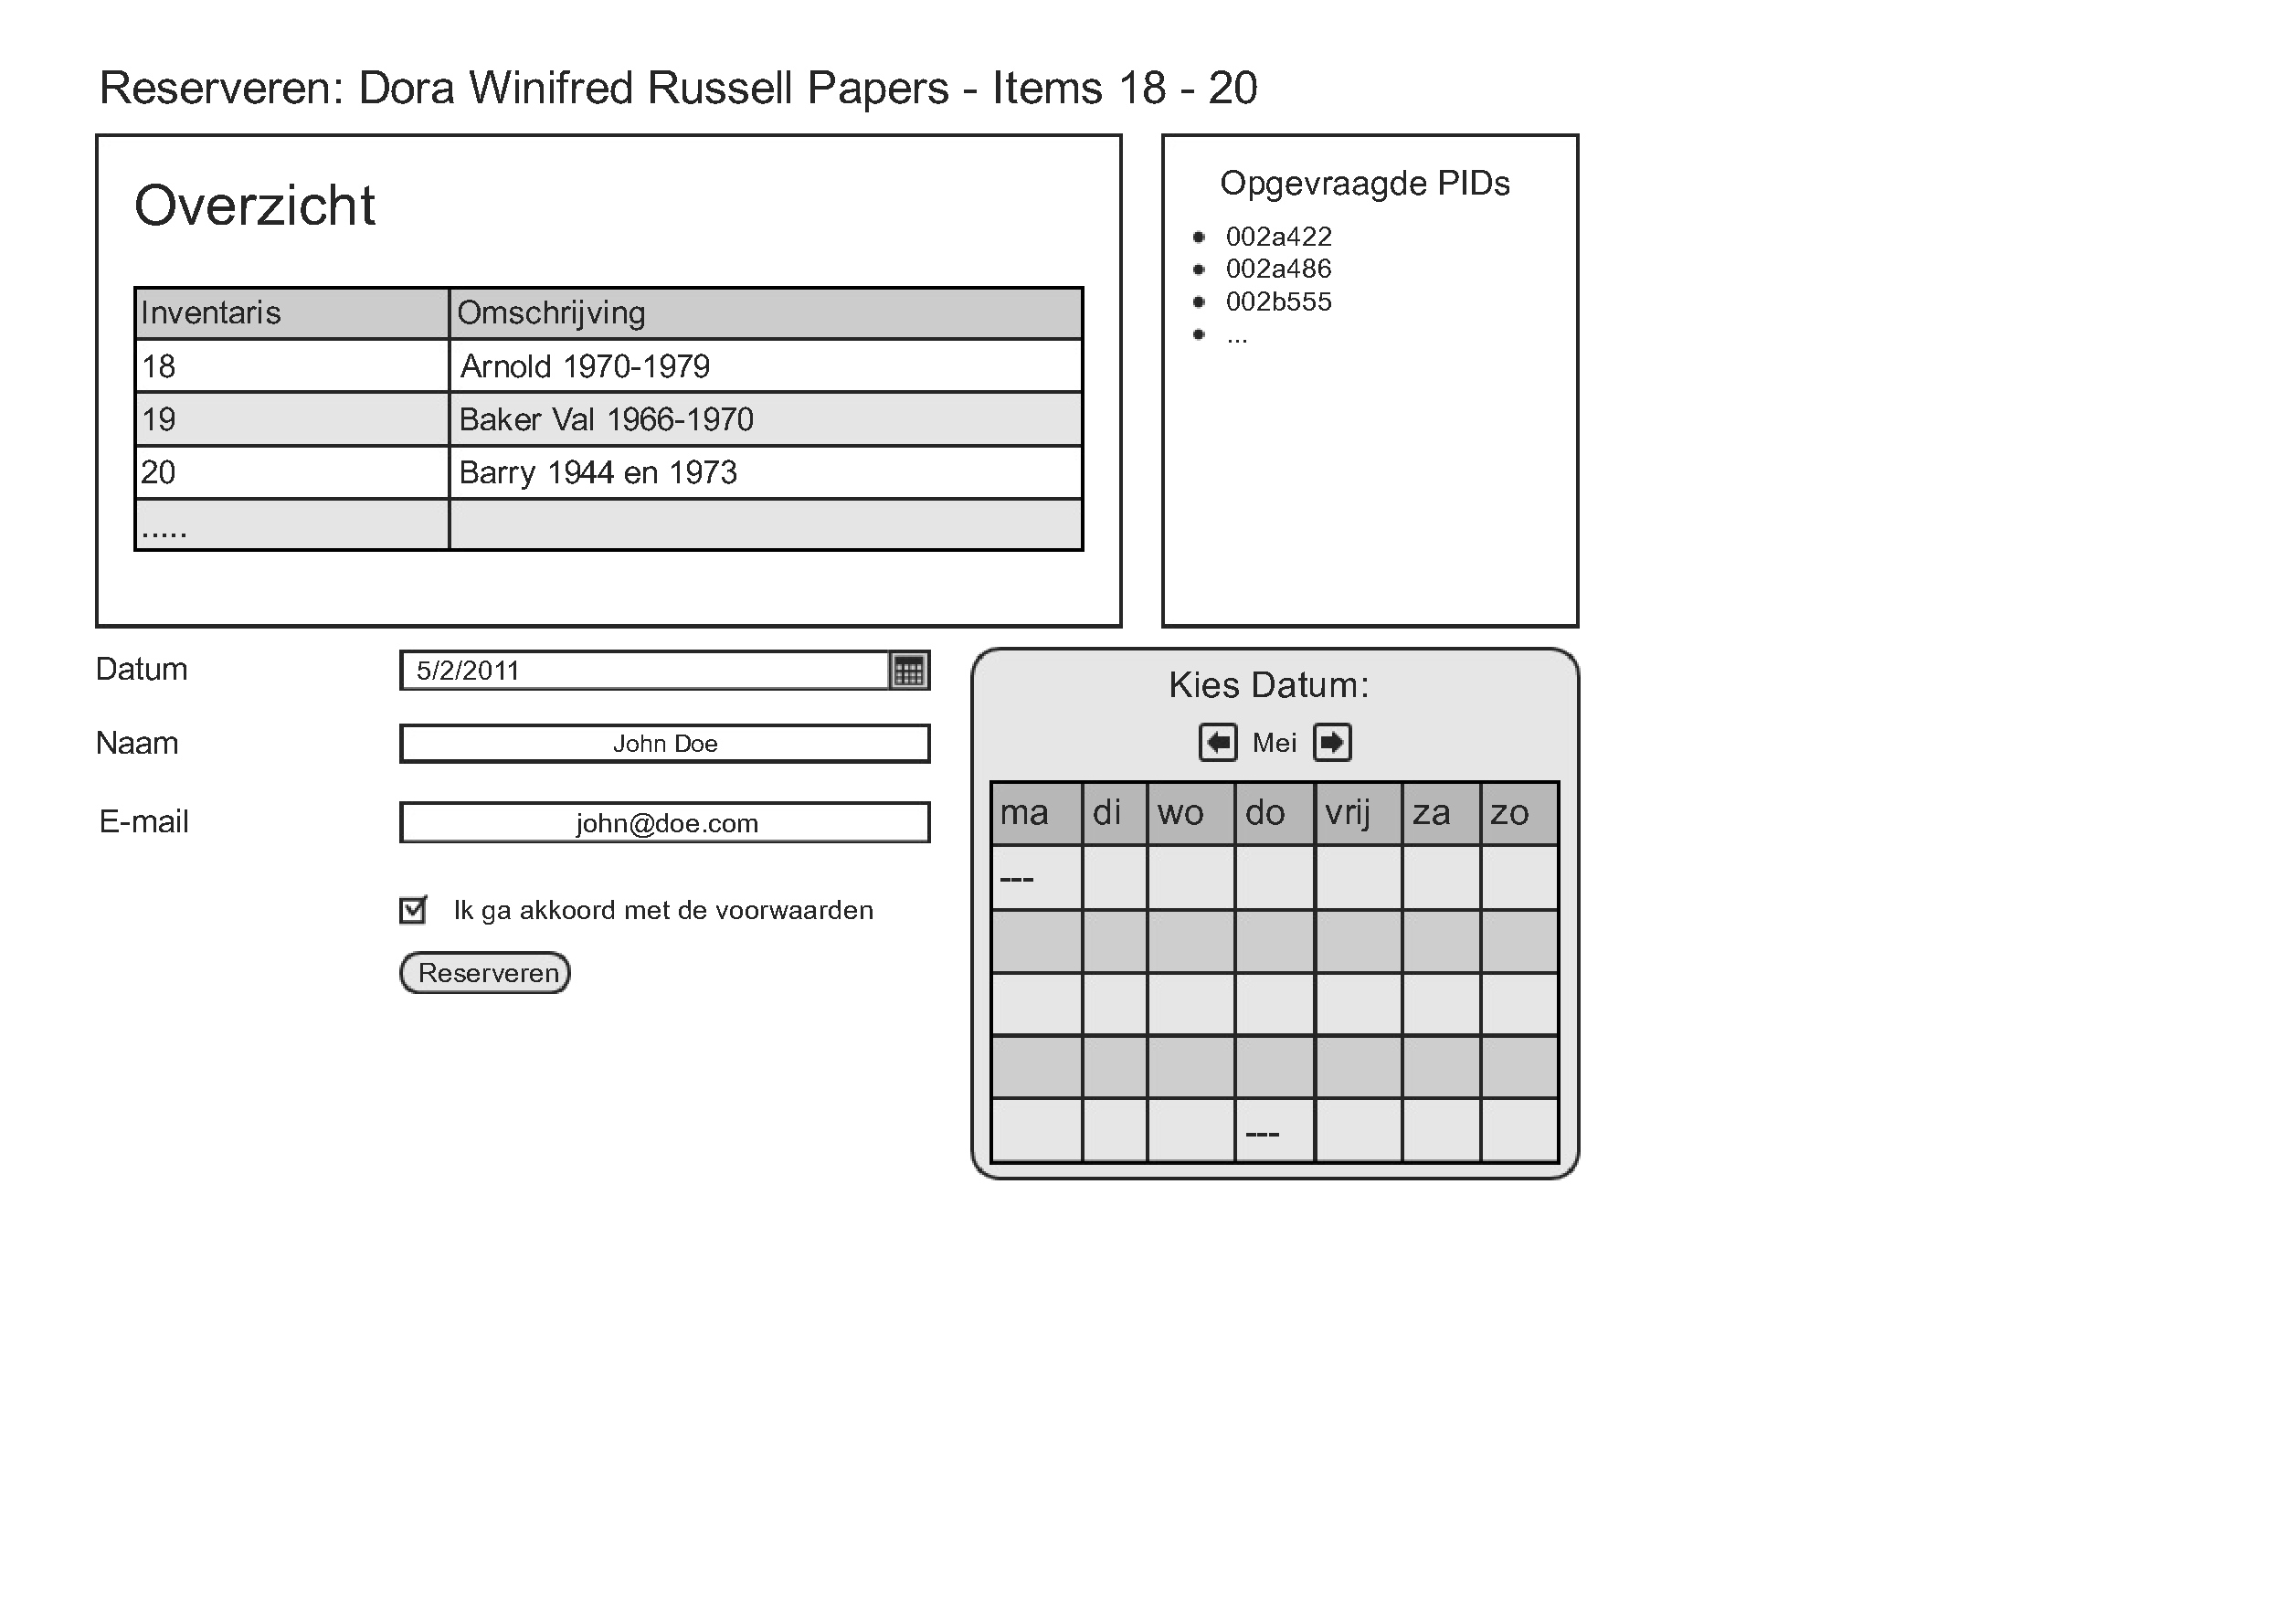
\includegraphics[totalheight=150mm,angle=90,page=1]{ui.pdf}
\end{figure}

\section{Reproducties bestellen}
\namedlabel{ui:bestel}{Reproducties bestellen}
\begin{figure}[H]
  \includegraphics[totalheight=150mm,angle=90,page=2]{ui.pdf}
\end{figure}

\section{Aanvraagoverzicht}
\namedlabel{ui:overzicht}{Aanvraagoverzicht}
\begin{figure}[H]
  \includegraphics[totalheight=150mm,angle=90,page=3]{ui.pdf}
\end{figure}


\section{Metadata Aanpassen}
\namedlabel{ui:metadata}{Metadata Aanpassen}
\begin{figure}[H]
  \includegraphics[height=170mm,page=5]{ui.pdf}
\end{figure}

\section{Aanvraag Toestemming}
\namedlabel{ui:aanvraag-toestemming}{Aanvraag Toestemming}
\begin{figure}[H]
  \includegraphics[totalheight=150mm,angle=90,page=6]{ui.pdf}
\end{figure}

\section{Toestemming Geven}
\namedlabel{ui:toestemming-geven}{Toestemming Geven}
\begin{figure}[H]
  \includegraphics[totalheight=150mm,angle=90,page=7]{ui.pdf}
\end{figure}

\printglossary[title=Verklarende Woordenlijst,toctitle=Verklarende Woordenlijst]

\appendix

\chapter{Toestandsdiagram voor Stukken}
\label{a:stuk-state}

\begin{figure}[H]
  \includegraphics[scale=0.8,trim=0mm 0mm 0mm 0mm]{status.pdf}
\end{figure}


\chapter{Workflows Afdeling Reproductie}
\label{a:workflows-repro}

\section{Huidige procedure}
\begin{figure}[H]
 \includegraphics[scale=0.7,trim=0mm 400mm 70mm 0mm,page=2]{e-levering.pdf}
\end{figure}
\section{Gewenste procedure}
\begin{figure}[H]
  \includegraphics[scale=0.7,trim=0mm 180mm 70mm 0mm,page=3]{e-levering.pdf}
\end{figure}
\end{document}
